\pagebreak

\mbox{}

\begin{figure}
\vspace*{-3cm}
\hspace*{-3.7cm}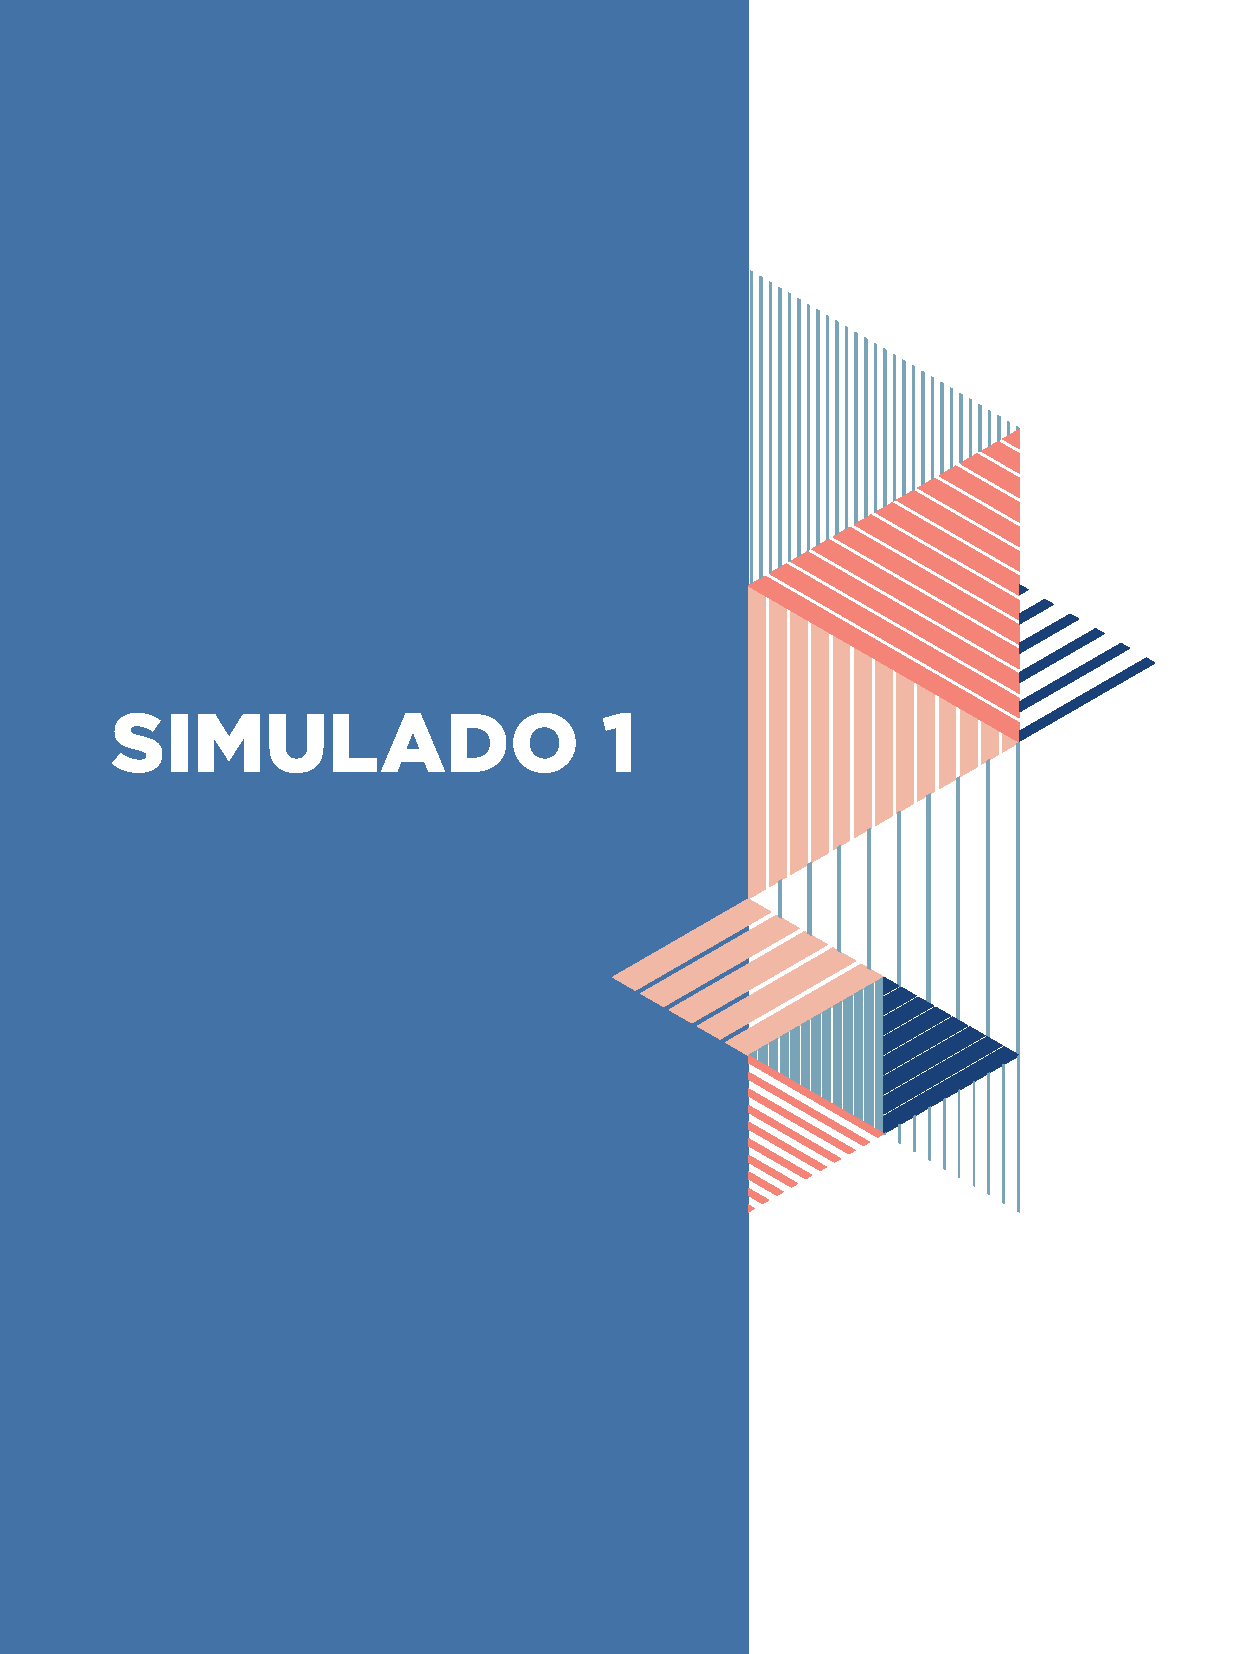
\includegraphics[scale=1]{../watermarks/1simulado9ano.pdf}
\end{figure}


\pagebreak

\section*{Simulado 1}

\num{1} Leia o texto.

\begin{quote}
\centering\textbf{Direito de ter direitos}

Cidadania --- uma palavra usada com frequência, mas que poucos entendem o
que significa --- quer dizer, em essência, a garantia por lei de viver
dignamente. É o direito de expressar as próprias ideias; de votar em
quem quiser sem nenhum tipo de constrangimento; de processar um médico
ou hospital por negligência ou imperícia; de devolver um produto
estragado e receber o dinheiro de volta; {[}...{]}

O direito de ter direitos foi uma conquista árdua da humanidade. No
Brasil, por exemplo, demorou muito tempo para que as pessoas tivessem o
direito de votar e escolher seus governantes. {[}...{]}

\fonte{Gilberto Dimenstein. \emph{O cidadão de papel:} a infância, a
adolescência e os Direitos Humanos no Brasil. São Paulo: Ática,
2012.}
\end{quote}

No texto, o trecho isolado por travessões pode ser interpretado como

\begin{escolha}
\item uma crítica.

\item um conselho.

\item uma dedução.

\item uma suposição.
\end{escolha}

\num{2} Analise o anúncio.

\begin{figure}[H]
\centering

\includegraphics[width=4.03125in,height=2.85231in]{./imgSAEB_8_POR/media/image28.png}
\caption{Disponível em: https://lucasdorioverde.mt.gov.br/site/noticias/campanha-de-vacinacao-antirrabica-sera-realizada-neste-sabado-07-5018/gallery.}
\end{figure}

A relação entre a imagem e a linguagem verbal é evidenciada, no texto da
campanha, pela presença de

\begin{escolha}
\item frases curtas.

\item frases nominais.

\item nomes de animais.

\item gírias de interação.
\end{escolha}

\num{3} Leia o texto.

\begin{quote}
Pescadores e caçadores são sempre os heróis de suas histórias {[}...{]}.
Quem quiser acreditar neste causo, aqui relatado, que acredite! Não sou
pescador, não sou caçador, sou apenas ouvinte. Ao ouvir este causo,
achei-o interessante e o escrevi, conforme segue nas linhas abaixo...

O causo se deu no Norte de Minas Gerais, numa cidadezinha rancheira,
onde o povo completava a sua alimentação com a pesca e com a caça.

Dizem que nessa cidadezinha existia um grande caçador, qual habilidade
queria passar ao filho primogênito de 15 anos. Ele procurava um modo de
parafrasear a famosa premissa popular: ``filho de peixe, peixinho é'',
tomando-a para ele como ``filho de caçador, caçadorzinho é''. {[}...{]}
\end{quote}

\fonte{RODRIGUES JÚNIOR, Francisco. \emph{Causos de Minas} -- Literatura:
memória, identidade e cultura mineira. Selo editorial: Independently
published, 2014 (fragmento).}

Em qual trecho texto o narrador se exime do compromisso com a veracidade
do causo que ele conta?

\begin{escolha}
\item ``Não sou pescador, não sou caçador, sou apenas ouvinte.''

\item ``Quem quiser acreditar neste causo, aqui relatado, que acredite!''

\item ``Ele procurava um modo de parafrasear a famosa premissa popular:''

\item ``O causo se deu no Norte de Minas Gerais, numa cidadezinha rancheira
{[}...{]}.''
\end{escolha}

\noindent Texto para as questões 4 e 5.

\begin{quote}
Fernando foi passar as férias na casa de Pedro, um amigo que mora há
muito tempo em outro
estado. Enquanto aproveitam a praia, eles conversam:

--- Nossa, que fome! Me dá uma bolacha aí!

--- Não tenho bolacha.

--- Então o que é isso que você tá comendo?

--- Biscoito.

--- Ah, tanto faz, o importante é matar a fome!

--- Tá bem, eu dou, mas você quer biscoito ou bolacha?

--- Não importa, tô com fome!

\fonte{Elaborado pelo autor.}
\end{quote}

\num{4} No diálogo, o fato de os amigos viverem em regiões diferentes faz com
que eles

\begin{escolha}
\item tenham opiniões diferentes sobre o sabor do alimento.

\item prefiram o biscoito ou a bolacha a qualquer outro lanche.

\item usem palavras diferentes para nomear o mesmo alimento.

\item discutam sobre a diferença de sabor entre o biscoito e a bolacha.
\end{escolha}

\num{5} O traço de humor do texto reside

\begin{escolha}
\item na indiferença de um dos amigos ao aceitar qualquer um dos lanches.

\item no pedido de um dos amigos ao querer comida num ambiente de praia.

\item no uso de abreviações de palavras numa situação que exigia
formalidade.

\item na atitude de um dos amigos ao fingir não conhecer a palavra usada
pelo colega.
\end{escolha}

\num{6} Analise os anúncios.

\begin{figure}[H]
\centering

\includegraphics[width=4.21103in,height=2.86458in]{./imgSAEB_8_POR/media/image29.png}
%\caption{Disponível em: https://pereirabarreto.sp.gov.br/noticias/saude/secretaria-municipal-de-saude-ira-vacinar-idosos-com-idade-entre-85-e-90-anos-neste-sabado.}
\end{figure}

\begin{figure}[H]
\centering

\includegraphics[width=4.21103in,height=2.86458in]{./imgSAEB_8_POR/media/image30.png}
%\caption{Disponível em: https://www.guarulhos.sp.gov.br/article/campanha-de-vacinacao-contra-polio-e-multivacinacao-e-prorrogada-ate-30-de-setembro.}
\end{figure}

Os dois textos têm em comum o fato de abordarem o mesmo assunto, mas sua
estratégia argumentativa se diferencia condicionada pelo

\begin{escolha}
\item assunto.

\item público-alvo.

\item meio de circulação.

\item objetivo comunicativo.
\end{escolha}

Texto para as questões 7 e 8.

\begin{quote}
Bom, inicialmente gostaria de agradecer a presença de todos. Para mim é
uma oportunidade importante, única e emotiva também, de mostrar o meu
trabalho. Enfim, é a função da minha vida. E gostaria de agradecer o
convite feito pelos professores e artistas. Vou fazer um depoimento
sobre a minha obra, sobre o meu trabalho. É a primeira vez que apresento
a grande maioria desses eslaides. Preparei uma seleção de imagens
focando a apresentação na produção de desenho, que é tema deste
seminário. Na verdade, meu surgimento como artista deu-se como
desenhista, e é bom que eu diga de início para, desde já, dar uma
resposta para essa questão do desenho como ponte: o desenho me colocou
no mundo, me colocou em contato com a minha comunidade, com as pessoas,
com o mundo em geral. {[}...{]}

\fonte{Disponível em: \emph{https://seer.ufrgs.br/RevistaValise/article/download/41375/26239.}
Acesso em: 16 fev. 2023. (Adaptado.)}
\end{quote}

\num{7} O trecho é a transcrição de uma apresentação oral feita em um seminário
universitário. Nesse contexto, o autor do texto privilegia o uso da
linguagem

\begin{escolha}
\item
  coloquial, buscando interagir com as pessoas da plateia.
\item
  técnica, usando termos da área profissional em que atua.
\item
  formal, promovendo a adequação à situação comunicativa.
\item
  regional, empregando o vocabulário da região dos ouvintes.
\end{escolha}

\num{8} O trecho ``Preparei uma seleção de imagens focando a apresentação na
produção de desenho, que é tema deste seminário'' contém o elemento
linguístico ``deste seminário'', que aponta para um elemento

\begin{escolha}
\item externo ao texto.

\item já citado no texto.

\item a ser citado no texto.

\item que pertence ao autor.
\end{escolha}

\num{9} Leia o poema.

\begin{quote}
Trago dentro do meu coração,

Como num cofre que se não pode fechar de cheio,

Todos os lugares onde estive,

Todos os portos a que cheguei,

Todas as paisagens que vi através de janelas ou vigias,

{[}...{]}

A entrada de Singapura, manhã subindo, cor verde,

O coral das Maldivas em passagem cálida,

{[}...{]}

E o Cabo da Boa Esperança nítido ao sol da madrugada...

E a Cidade do Cabo com a Montanha da Mesa ao fundo...

\fonte{Fernando Pessoa. Disponível em: \emph{http://www.dominiopublico.gov.br/download/texto/pe000010.pdf.}
Acesso em: 11 fev. 2023.}
\end{quote}

Como tema central, o eu lírico expressa no poema

\begin{escolha}
\item a saudade da sua terra natal.

\item as lembranças das suas viagens.

\item a vontade de conhecer o mundo.

\item o gosto pelas belezas da natureza.
\end{escolha}

\num{10} Analise o anúncio.

\begin{figure}[H]
\centering

\includegraphics[width=4.21103in,height=2.86458in]{./imgSAEB_8_POR/media/image31.png}
%\caption{Disponível em: https://www.amapa.gov.br/ler_noticia.php?slug=1407/julho-amarelo-prevencao-diagnostico-precoce-e-tratamento-sao-essenciais-nos-casos-de-hepatite}
\end{figure}

A estratégia de persuasão empregada no texto enfatiza

\begin{escolha}
\item
  a forma de contágio da doença.
\item
  os integrantes do grupo de risco.
\item
  a ausência de sintomas da doença.
\item
  os fatores de risco para o contágio.
\end{escolha}

\num{11} Leia os textos.

\textbf{TEXTO I}

\begin{quote}
\centering\textbf{Estudo alerta para vacinação infantil abaixo da meta no estado
do Rio}

\emph{Prefeituras têm até 2024 para fornecer dados ao Ministério da
Saúde}

As metas de cobertura vacinal de crianças menores de cinco anos não
foram atingidas no estado do Rio de Janeiro para nenhuma das vacinas do
calendário infantil de 2022, alerta levantamento preliminar divulgado
nesta terça-feira (27) pela Fundação Oswaldo Cruz (Fiocruz).

Apesar de ser o segundo estado mais rico do país, o Rio de Janeiro
também está abaixo da cobertura média nacional de todas as vacinas, não
chegando a atingir metade do público-alvo no caso das proteções contra
poliomielite, difteria, tétano, coqueluche, hepatite B, pneumonia e
meningite bacterianas. {[}...{]}

Mesmo que alguns municípios consigam atingir as metas para algumas
vacinas com a atualização dos dados, a coordenadora do Observa Infância,
Patricia Boccolini, avaliou que o cenário geral do estado continuará
sendo de baixas coberturas. {[}...{]}

\fonte{Disponível em: \emph{https://agenciabrasil.ebc.com.br/saude/noticia/2022-12/estudo-alerta-para-vacinacao-infantil-abaixo-da-meta-no-estado-do-rio.}
Acesso em: 13 fev. 2023.}
\end{quote}


\textbf{TEXTO II}

\begin{figure}[H]
\centering
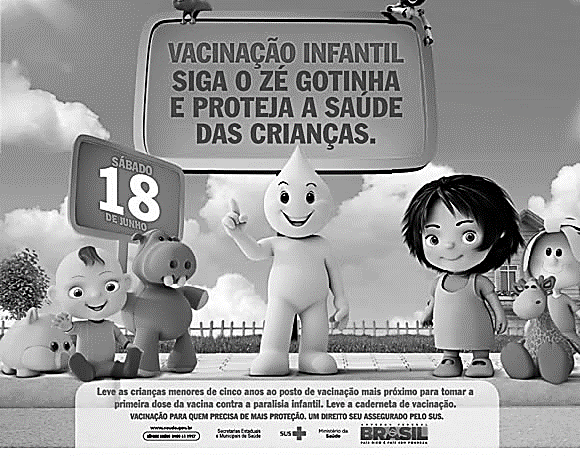
\includegraphics[width=3.15625in,height=2.48418in]{./imgSAEB_8_POR/media/image32.png}
%\caption{https://chc.org.br/wp-content/uploads/2011/11/z%c3%a9-gotinha.jpg}
\end{figure}


Comparando-se os dois textos, conclui-se que o texto II cumpre, em
relação à situação noticiada no texto I, a função de

\begin{escolha}
\item apresentar o personagem Zé Gotinha e seus amigos ao público infantil.

\item convidar as crianças a seguirem as redes sociais do personagem Zé
Gotinha.

\item divulgar as campanhas de vacinação infantil do governo e atrair a
população.

\item entreter o público infantil com ilustrações sobre vacinação adequadas
à faixa etária.
\end{escolha}

\num{12}

\textbf{TEXTO I}

\textbf{CBF define punição por racismo em competições nacionais; clubes poderão perder pontos}

\textit{Medida já foi incluída no Regulamento Geral de Competições (RGC) de 2023 e passará a valer na Copa do Brasil, que começa semana que vem}


\textbf{TEXTO II}

\textbf{CBF acerta ao determinar punição a racismo em estádios no Brasil}

\textit{A decisão da CBF, inédita, chega até tarde, mas ainda assim precisa ser comemorada; clubes terão de pagar multa e podem até perder pontos em caso de racismo}

Ao se deparar com os fragmentos de texto I e II, sobre o mesmo assunto,
o leitor pode prever que a finalidade deles, respectivamente, é

\begin{escolha}
\item informar e opinar.

\item criticar e informar.

\item opinar e denunciar.

\item reivindicar e conscientizar.
\end{escolha}

\num{13} Leia o texto.

\textbf{Defesa Civil alerta para chuvas intensas em SP no carnaval}

\begin{quote}
O carnaval em São Paulo terá chuvas intensas, segundo alerta da Defesa
Civil Estadual. A previsão meteorológica é que o volume alcance de 80
milímetros a 250 milímetros até domingo (19). O litoral norte do estado
deve ser o mais impactado. A Baixada Santista, Serra da Mantiqueira,
Vale do Ribeira e Itapeva podem ter até 150 milímetros de chuvas. Com o
solo já encharcado, há risco de deslizamentos em regiões de encosta.

{[}...{]}

\fonte{
Disponível em: \url{https://agenciabrasil.ebc.com.br/geral/noticia/2023-02/defesa-civil-alerta-para-chuvas-intensas-no-carnaval-em-sao-paulo.}
Acesso em: 17 fev. 2023 (fragmento).}
\end{quote}

A finalidade do texto é informar a previsão do tempo. As formas verbais
``alcance'', ``deve ser'' e ``podem ter'' estão empregadas nos tempos e
modos verbais adequados para

\begin{escolha}
\item quantificar o volume de chuvas que é esperado para o período de
carnaval.

\item recomendar cautela e atenção à população que vive nas regiões
mencionadas.

\item ressaltar o alerta de chuvas intensas que foi emitido pela Defesa
Civil Estadual.

\item exprimir a ideia de possibilidade e hipótese do que pode acontecer
com o clima.
\end{escolha}

Texto para as questões 14 e 15.

\begin{quote}
--- Gosto muito de ouvir você, Olívia. Sei que vou me esquecer... Espero
que você não se importe de repetir sua história outras vezes. Você se
importa?

--- Não.

--- Ouvirei sempre como se fosse a primeira vez. Isso é o que posso
prometer. E não é pouco, viu? A primeira vez tem sempre os melhores
ouvidos. Quando ouvi ``Erbarme dich'', de Bach, pela primeira vez...
Você conhece essa música?

--- Acho que não... talvez.

\fonte{MADEIRA, Carla. \emph{A natureza da mordida.} 1.ed. Rio de Janeiro:
Record, 2022 (fragmento).}
\end{quote}

\num{14} No diálogo, a personagem é interpelada duas vezes. Em relação à segunda
pergunta que lhe é feita, sua resposta expressa

\begin{escolha}
\item hesitação.

\item desinteresse.

\item constrangimento.

\item desconhecimento.
\end{escolha}


\num{15} A figura de linguagem empregada em ``A primeira vez tem sempre os
melhores ouvidos'' introduz a intenção de

\begin{escolha}
\item expressar a opinião da locutora em relação à melodia de Bach.

\item recomendar a apreciação da melodia ``Erbarme dich'', de Bach.

\item valorizar o esforço da personagem Olívia de recontar sua história.

\item desculpar-se pelo esquecimento da história de vida contada antes.
\end{escolha}
